%=========================================================
%---- fase conceitual ------------------------------------
%=========================================================
%\chapter{BASIS OF DESIGN}
%\label{chap:bod}
%
%%---- fase conceitual ------------------------------------
%\section{Requisitos do cliente}
%\label{sec:reqcli}
%
%%---- fase conceitual ------------------------------------
%\section{Estudo do estado da arte}
%\label{sec:sota}
%
%%---- fase conceitual ------------------------------------
%\subsection{Benchmarking}
%\label{sec:bnchmkg}
%
%%---- fase conceitual ------------------------------------
%\section{Ambiente de operação}
%\label{sec:ambopt}
%
%%---- fase conceitual ------------------------------------
%\section{Normas}
%\label{sec:normas}


\chapter{MANIPULADOR SUBAQUÁTICO - \textit{PoC}}
\label{chap:manisub-s}
Este capítulo tem o objetivo de apresentar a concepção do desenvolvimento de várias funcionalidades de um manipulador subaquático e que seja capaz de reconhecer alvos e consequentemente realizar tarefas de forma autônoma, mesmo que seu frame de localização seja alterado durante a missão. É importante salientar que o desenvolvimento deste projeto procura estabelecer uma prova de conceito para que estas funcionalidades sejam testadas mesmo antes de um envolvimento num ambiente subaquático.

As funcionalidades a serem testadas em laboratório são: 
\begin{enumerate}
	\item percepção do manipulador: esta funcionalidade tem por objetivo reconhecer um marcador tipo \textit{aprilTag} (Figura \ref{fig:apriltag}) e identificar a posição de atuação para a trajetória da missão.
	\item navegação da plataforma móvel: objetivo é fornecer comandos para realização de movimentos tanto em manual com em rotas pré-programadas, nestas rotas pontos aleatórios serão gerados simulando distúrbios marinhos que podem ocorrem em ROVs.
	\item planejamento da trajetória: diante da informação da posição a ser realizada e tendo as perturbações geradas, o planejamento será capaz de reposicionar o \textit{end-effector} do manipulador para atender a trajetória do mesmo.
	\item atuação do manipulador: o objetivo principal desta funcionalidade será o de realizar o comando de apertar o botão localizado pela primeira funcionalidade abordada.
\end{enumerate}

%------ picture -------------
%\begin{sidewaysfigure*}
\begin{figure}[H] 
  \begin{center} 
  	
\includegraphics[width=0.4 \textwidth]{images/apriltag.png} 
  \end{center} 
  \caption{Exemplo de um marco fiducial (apriltag).} 
  %\legend{Fonte: os autores.} 
  \label{fig:apriltag} 
\end{figure}
%\end{sidewaysfigure*}
%----------------------------



%\section{Base of design}
\section{Base do desenvolvimento}
\label{sec:bod-s}
Um dos pontos importantes para uma pesquisa inicial de uma determinada tecnologia, é poder testar alguns funcionalidades da ideia principal com um mínimo de recursos necessários para o desenvolvimento de um protótipo. Neste projeto para testar várias das funcionlidades apresentadas na introdução do capítulo \ref{chap:manisub-s}, foi considerado analogamente dois elementos para simular tanto o ROV quanto o manipulador subaquático. Para simular as perturbações do ambiente aquático, foi idealizado desenvolver a PoC num piso irregular, que pudesse a todo tempo alterar o psocionamento da base do manipulador.

De forma descritiva, a Figura \ref{fig:manipoc} apresenta uma ideia sobre o teste a ser realizado

%------ picture -------------
%\begin{sidewaysfigure*}
\begin{figure}[H] 
  \begin{center} 
  	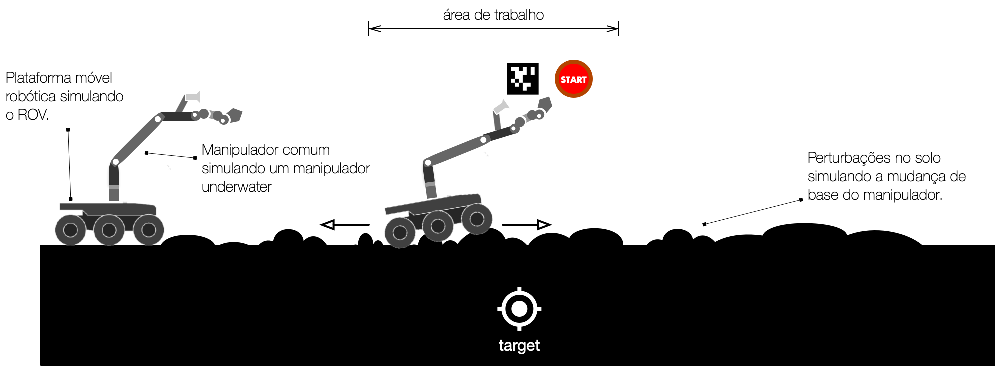
\includegraphics[width=1 \textwidth]{images/ManiSub_PoC.png} 
  \end{center} 
  \caption{Modelo representativo da prova de conceito.} 
  %\legend{Fonte: os autores.} 
  \label{fig:manipoc} 
\end{figure}
%\end{sidewaysfigure*}
%----------------------------

Para a demonstração da missão que o manipulador desenvolverá autonomamente, foi idealizado uma determinada região fixa para a plataforma móvel com um ponto referencial de fixação simulando o processo de ancoragem para o ROV, tendo estabelecido a ancoragem o sistema ficará sujeito às perturbações, que poderão ocorrer de forma aleatório ou não, dependendo somente da programação inicial que será levada em consideração na realização dos testes.

A próxima tarefa, o manipulador fará uma busca de reconhecimento com o intuito de encontrar um determinado marcador (Figura \ref{fig:apriltag}), que será capaz de informar ao manipulador para qual ponto da trajetória o mesmo deverá ir. Com a informação do ponto determinada, o sistema do manipulador deverá realizar cálculos de controle e de cinemática inversa em tempo real para a trajetória a ser desenvolvida. Este planejamento deverá, ao final do projeto, ser autônoma e precisa.

Com isso, o manipulador será capaz de realizar a missão para o qual foi planejado, que no caso deste projeto é o de apertar um botão, girar uma chave de emergência, inserir um pino no painel, realizar uma trajetória linear e uma circular, com o intuito de simular um processo de limpeza e uma inspeção em um \textit{pipeline} respectivamente.


%%%%%%% descrever a ideia

\subsection{Adaptação às condições operacionais}
\label{ssec:adap}
No desenvolvimento da prova de conceito é levada em consideração características operacionais que estejam em de acordo com a norma API RP 17H para o uso de ROVs de intervenção conforme Tabela xxx. Estas características são consideradas especificamente na simulação da prova de conceito. 




%
%%---- fase conceitual ------------------------------------
\subsection{Requisitos do cliente}
\label{ssec:reqcli-s}
A ideia apresentada na introdução desta seção tem como objetivo suprir com entendimento os requisitos levantados e impostos ao time de desenvolvimento quando do início do proejto.
Entendendo estas necessidades apontadas pelo cliente durante as reuniões realizadas, e analisando o plano de trabalho estabelecido, pode-se listar os seguintes requisitos primordiais para a realização deste projeto:
\begin{itemize}
	\item projetar, construir e demonstrar uma prova de conceito em laboratório para simular a automação de operações com ROVs que utilizam braços manipuladores;
	\item desenvolver um estudo de viabilidade técnico-econômica para automatizar algumas operações com ROVs, contendo os seguintes tópicos:
		\begin{itemize}
			\item Relação de operações usuais de ROVs e seus manipuladores;
			\item Estudo do estado da arte de ROVs;
			\item Estudo do estado da arte de manipuladores subaquáticos;
			\item Avaliação da complexidade das operações realizadas por ROVs e seus manipuladores;
			\item Avaliação do custo operacional dos manipuladores subaquáticos e o impacto nos custos totais das operações com ROVs;
			\item Estimação da redução de custos e tempos de operação quando da implementação da automação dos manipuladores;
			\item Estimação da redução dos riscos humanos principalmente referentes à prática de mergulho nas operações;
			\item Análise de risco da implementação da automação dos manipuladores;
			\item Avaliação da prontidão tecnológica para implementação da automação dos manipuladores;
			\item Análise de viabilidade técnico-econômica e impacto na operação da empresa.
		\end{itemize}
	\item elaborar um plano de trabalho, em decorrência da análise realizada no estudo de viabilidade, com o intuito de estabelecer um \textit{road map} para a aplicação de tecnologias apontadas no estudo.
\end{itemize}

Com três grandes entregáveis: prova de conceito, estudo de viabilidadse, e o plano de trabalho para o protótipo; o projeto estabelecerá respostas para cada requisito apresentado. O estudo de viabilidade foi iniciado com o levantamento dos requisitos e com a elaboração de questões a serem indagadas à equipe da PETROBRAS e aos fornecedores de equipamentos. Estas questões são apresentadas de forma preliminar no Apêndice \ref{ape:quest}, porém vale ressaltar que melhorias serão apontadas quando da realização do workshop no CENPES e no campo operacional de Macaé - RJ.

\section{Testes iniciais da simulação}
\label{sec:tstsim}
Para a prova de conceito que validará o controle de posição e trajetória de um manipulador submetido a perturbações 3D; uma forma de acelerar o desenvolvimento e focar nas funcionalidades requeridas para o manipulador é usar uma plataforma móvel que já esteja integrada com um manipulador. Além disso se o conjunto possuir câmera e unidade de processamento que possa processar algoritmos de mapeamento de imagens será um diferencial grande para o desenvolvimento. No entanto antes disso tudo, é necessário simular estes processos antes mesmo de submerter a implementação física.

Neste início de desenvolvimento, os compoonentes selecionados foram a plataforma robótica móvel do fabricante Clearpath  (Figura \ref{fig:jackal}) e o manipulador do fabricante Kinova (Figura \ref{fig:jaco2}).
%------ picture -------------
%\begin{sidewaysfigure*}
\begin{figure}[H] 
  \begin{center} 
  	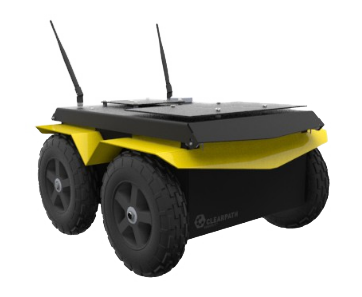
\includegraphics[width=0.5 \textwidth]{images/jackal.png} 
  \end{center} 
  \caption{Plataforma robótica móvel - Jackal.} 
  %\legend{Fonte: os autores.} 
  \label{fig:jackal} 
\end{figure}
%\end{sidewaysfigure*}
%----------------------------

%------ picture -------------
%\begin{sidewaysfigure*}
\begin{figure}[H] 
  \begin{center} 
  	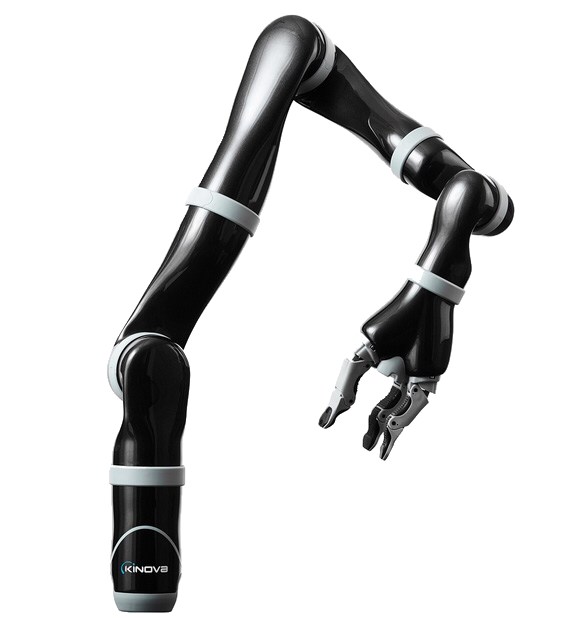
\includegraphics[width=0.4 \textwidth]{images/jaco2.png} 
  \end{center} 
  \caption{Manipulador - Jaco 2.} 
  %\legend{Fonte: os autores.} 
  \label{fig:jaco2} 
\end{figure}
%\end{sidewaysfigure*}
%----------------------------

Diante das informações obtidas dos fabricantes foi possível parametrizar as variáveis necessárias para que a simulação fosse a mais próxima do real. De forma a testar a idea principal no uso de manipuladores quando os mesmos são submetidos a perturbações e que a sua base é alterada aleatoriamente foi pensado em elaborar uma simulação utilizando o Pybullet \cite{pybullet} , que é uma plataforma em tempo real que simula as propriedade físicas de materiais de mecanismos robóticos.

O foco principal do teste foi elaborar uma trajetória pré-programada do manipulador e que durante o processo de trajetória sofresse uma perturbação em sua base.

O resultado esperado era o desempenho da trajetória na realização da missão, mostrando se eficaz na primeira tentativa, que era o de simplesmente permanecer no ponto esperado (Figura \ref{fig:jjsim}).
%------ picture -------------
%\begin{sidewaysfigure*}
\begin{figure}[H] 
  \begin{center} 
  	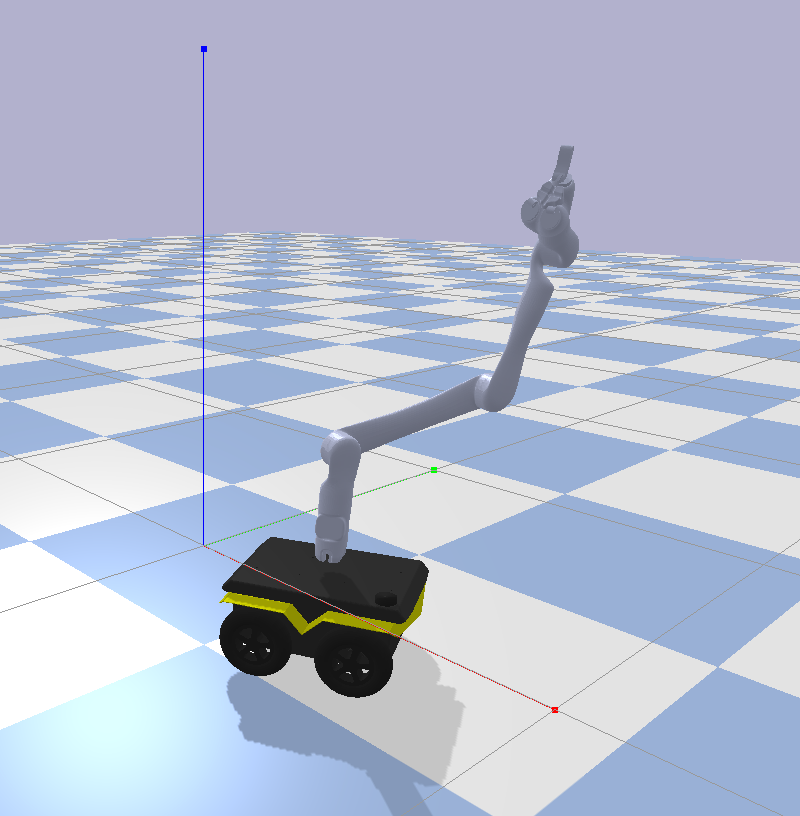
\includegraphics[width=0.4 \textwidth]{images/jjsim.png} 
  \end{center} 
  \caption{Modelo do sistema para a simulação.} 
  %\legend{Fonte: os autores.} 
  \label{fig:jjsim} 
\end{figure}
%\end{sidewaysfigure*}
%----------------------------

Com o resultado alcançado com o primeiro teste, em que o \textit{end-effector} tende a permanecer no ponto designado inicialmente, foi elaborado o segundo teste no qual requereria do \textit{end-effector} uma determinada tarefa a ser realizada mesmo tendo a base do manipulador alterada aleatoriamente.

Neste segundo teste, que está sendo apresentado na Figura \ref{fig:jjsimula} tem a intenção de apresentar uma certa sequência dos eventos realizados durante a simulação.
A tarefa desempenhada pelo \textit{end-effector} do manipulador foi o de descrever uma trajetória circular num determinado ponto.
Na Figura \ref{fig:jjsim1-1} o manipulador está na posição inicial da trajetória estipulada na missão, como consequência do evento o manipulador deve realizar uma trajetória que descreve uma circunferência no espaço (Figura \ref{fig:jjsim1-2}). Consequentemente após receber uma determinada perturbação de mudança na base do manipulador, o \textit{end-effector} permanece realizando a trajetória circular, conforme apresentado na Figura \ref{fig:jjsim1-3}.

O resultado do teste mostrou-se compatível com a ideia inicial em permanecer desenvolvendo a trajetória mesmo tendo a sua base fixa sofrendo perturbações em seus eixos.

\begin{figure}[ht]
	\begin{minipage}[t]{0.3\linewidth}
		%		\centering
		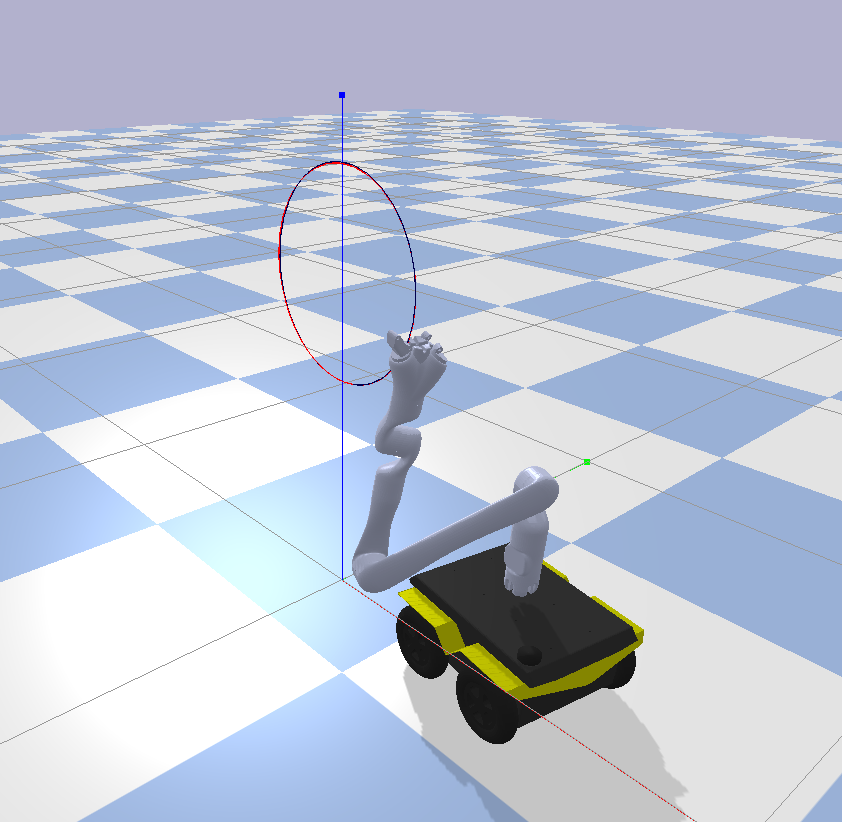
\includegraphics[width=1\textwidth]{images/jjsim1-1.png}
		\subcaption{Ponto inicial.}
		\label{fig:jjsim1-1}
	\end{minipage}
	\hfill
	\begin{minipage}[t]{0.3\linewidth}
		%		\centering
		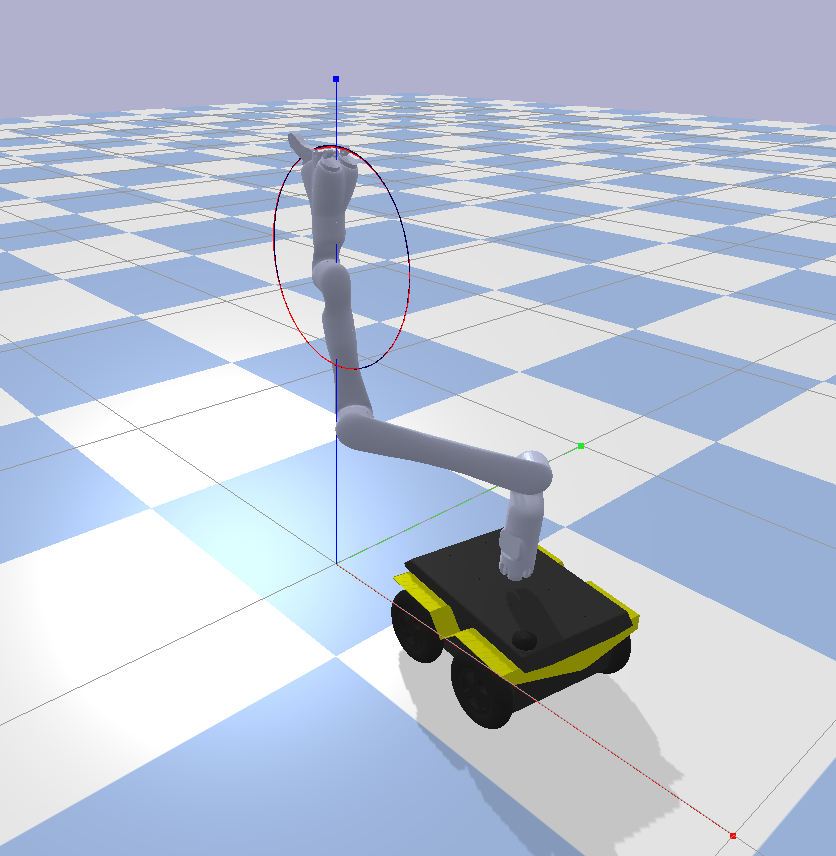
\includegraphics[width=1\textwidth]{images/jjsim1-2.png}
		\subcaption{Percorrendo um círculo.}
		\label{fig:jjsim1-2}
	\end{minipage}
	\hfill
	\begin{minipage}[t]{0.3\linewidth}
		%		\centering
		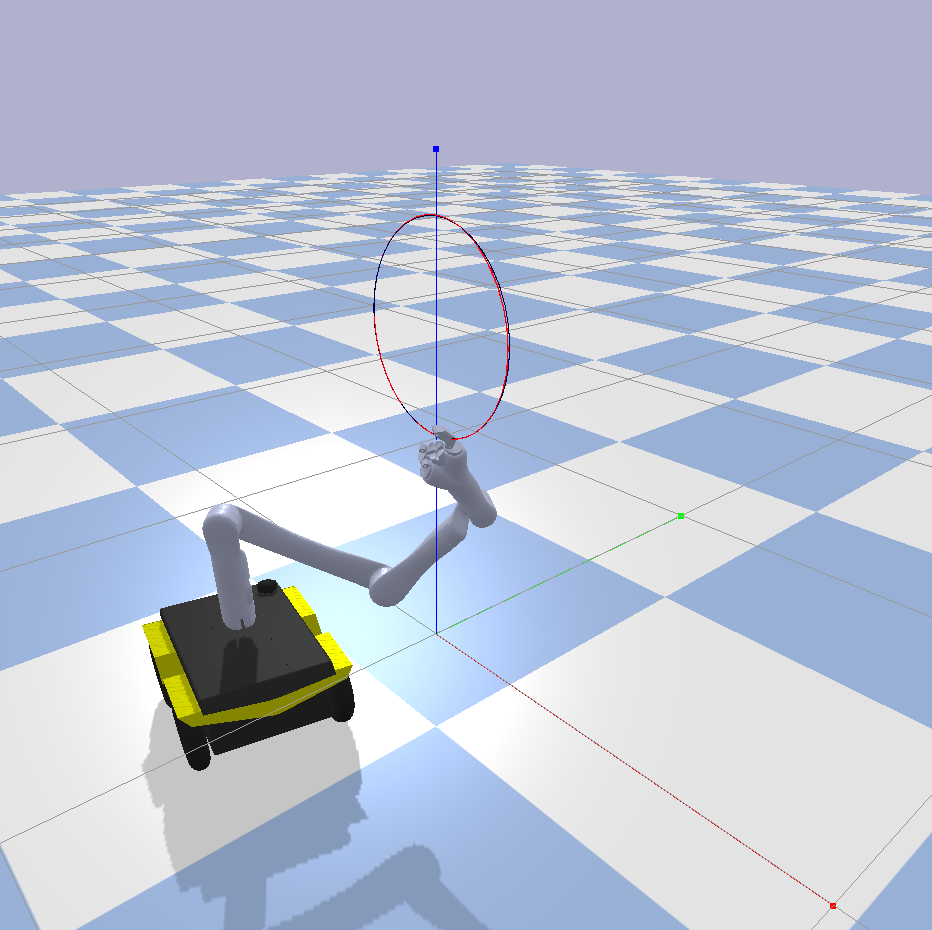
\includegraphics[width=1\textwidth]{images/jjsim1-3.png}
		\subcaption{Sistema com a base em um outra posição.}
		\label{fig:jjsim1-3}
	\end{minipage}  
	\caption{Simulação do sistema utilizando o PyBullet.}
	%\legend{Fonte: Própria.}
	\label{fig:jjsimula}
\end{figure}


%%---- fase conceitual ------------------------------------
%\section{Estudo do estado da arte}
%\label{sec:sota}
%
%
%
%%%---- fase conceitual ------------------------------------
%%\subsection{Benchmarking}
%%\label{sec:bnchmkg}
%
%%---- fase conceitual ------------------------------------
%\subsection{Ambiente de operação}
%\label{ssec:ambopt-s}

%%---- fase conceitual ------------------------------------
%\subsection{Normas aplicadas}
%\label{ssec:normas-s}


%\section{Análise técnica}
%\label{sec:an-tec-s}
%
%\subsection{Análise da avaliação da prontidão tecnológica}
%\label{sec:an-trl-s}
%
%
%\section{Análise econômica}
%\label{sec:an-eco-s}
%
%\subsection{Análise de risco}
%\label{sec:an-rsk-s}
%



